\documentclass[11pt]{article}
\usepackage[textwidth=18.0cm, textheight=23.0cm, top=2.0cm]{geometry}
\usepackage{pst-all}
\usepackage{amssymb}
\usepackage{tikz}
\usepackage{underscore}\begin{document}
\pagestyle{empty}


ClassName: \underline{\textbf{Class_03.2bp-24}}
\par
BinSize: \underline{\textbf{40 × 40}}
\par
ReduceSize: \underline{\textbf{40 × 40}}
\par
TypeNum: \underline{\textbf{60}}
\par
Num: \underline{\textbf{60}}
\par
OutS: \underline{\textbf{19200}}
\par
InS: \underline{\textbf{17407}}
\par
Rate: \underline{\textbf{0.907}}
\par
UB: \underline{\textbf{12}}
\par
LB0: \underline{\textbf{12}}
\par
LB: \underline{\textbf{12}}
\par
LBWithCut: \underline{\textbf{12}}
\par
NodeCut: \underline{\textbf{0}}
\par
ExtendedNodeCnt: \underline{\textbf{1}}
\par
GenNodeCnt: \underline{\textbf{1}}
\par
PrimalNode: \underline{\textbf{0}}
\par
ColumnCount: \underline{\textbf{12}}
\par
TotalCutCount: \underline{\textbf{0}}
\par
RootCutCount: \underline{\textbf{0}}
\par
LPSolverCnt: \underline{\textbf{1}}
\par
PricingSolverCnt: \underline{\textbf{0}}
\par
BranchAndBoundNum: \underline{\textbf{1}}
\par
isOpt: \underline{\textbf{true}}
\par
TimeOnInitSolution: \underline{\textbf{600.000 s}}
\par
TimeOnPrimal: \underline{\textbf{0.000 s}}
\par
TimeOnPricing: \underline{\textbf{0.000 s}}
\par
TimeOnRmp: \underline{\textbf{0.063 s}}
\par
TotalTime: \underline{\textbf{600.391 s}}
\par
\newpage


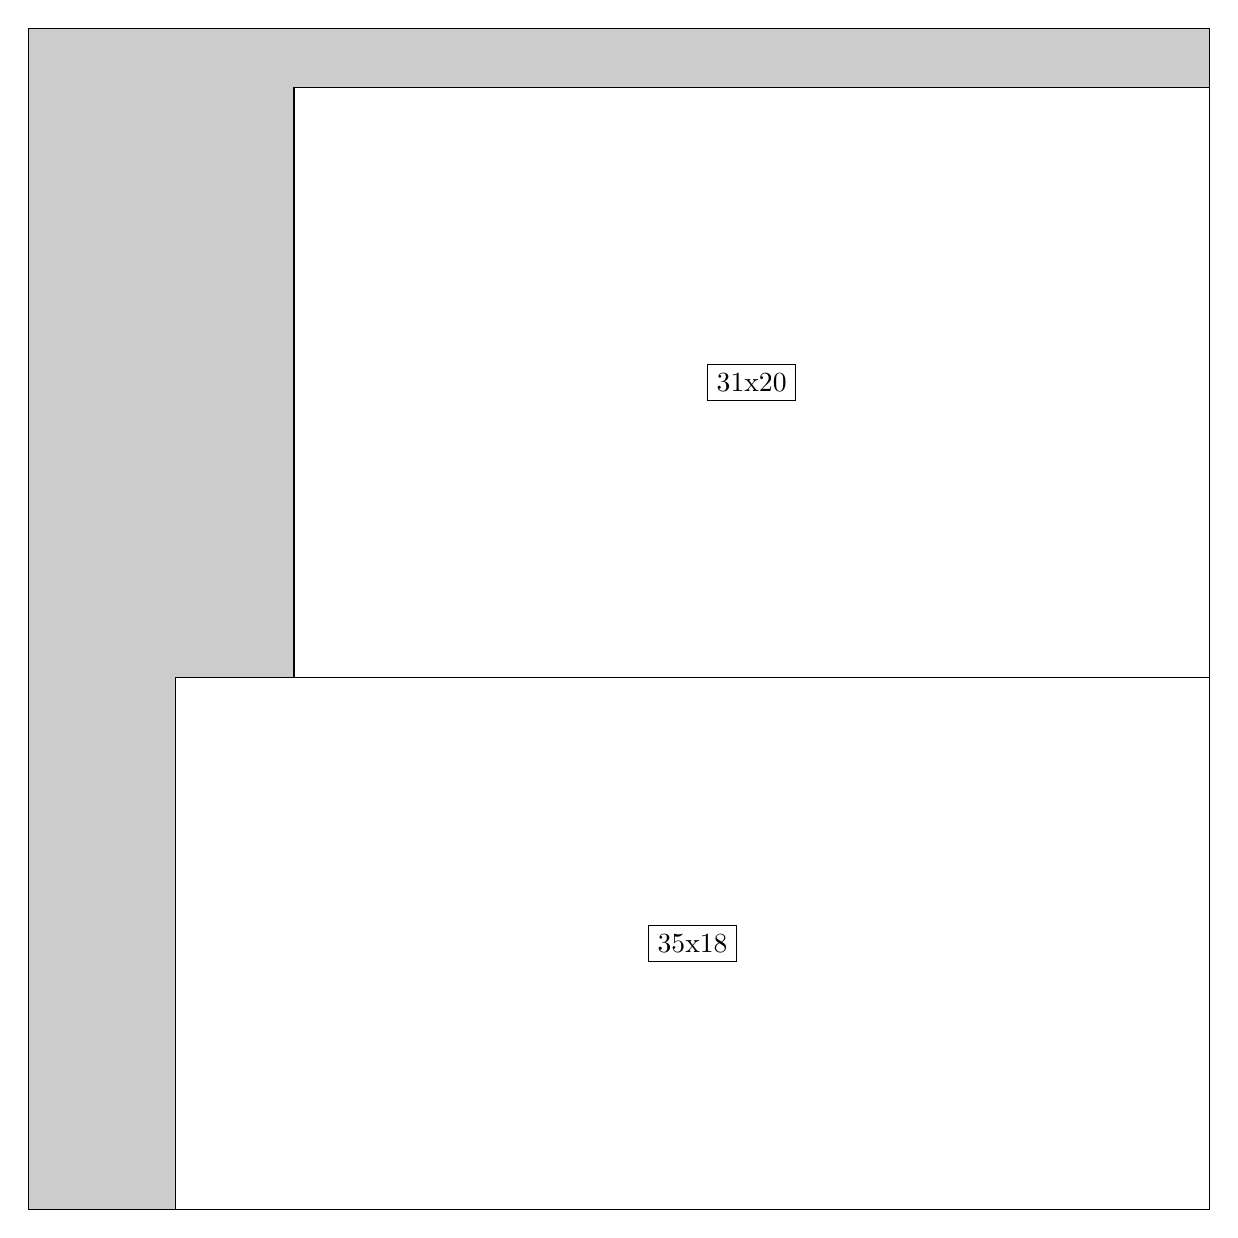
\begin{tikzpicture}[shorten >=1pt,scale=1.0,every node/.style={scale=1.0},->]
\tikzstyle{vertex}=[circle,fill=black!25,minimum size=14pt,inner sep=0pt]
\filldraw[fill=gray!40!white, draw=black] (0,0) rectangle (15.0,15.0);
\foreach \name/\x/\y/\w/\h in {35x18/1.875/0.0/13.125/6.75,31x20/3.375/6.75/11.625/7.5}
\filldraw[fill=white!40!white, draw=black] (\x,\y) rectangle node[draw] (\name) {\name} ++(\w,\h);
\end{tikzpicture}


w =35 , h =18 , x =5 , y =0 , v =630
\par
w =31 , h =20 , x =9 , y =18 , v =620
\par
\newpage


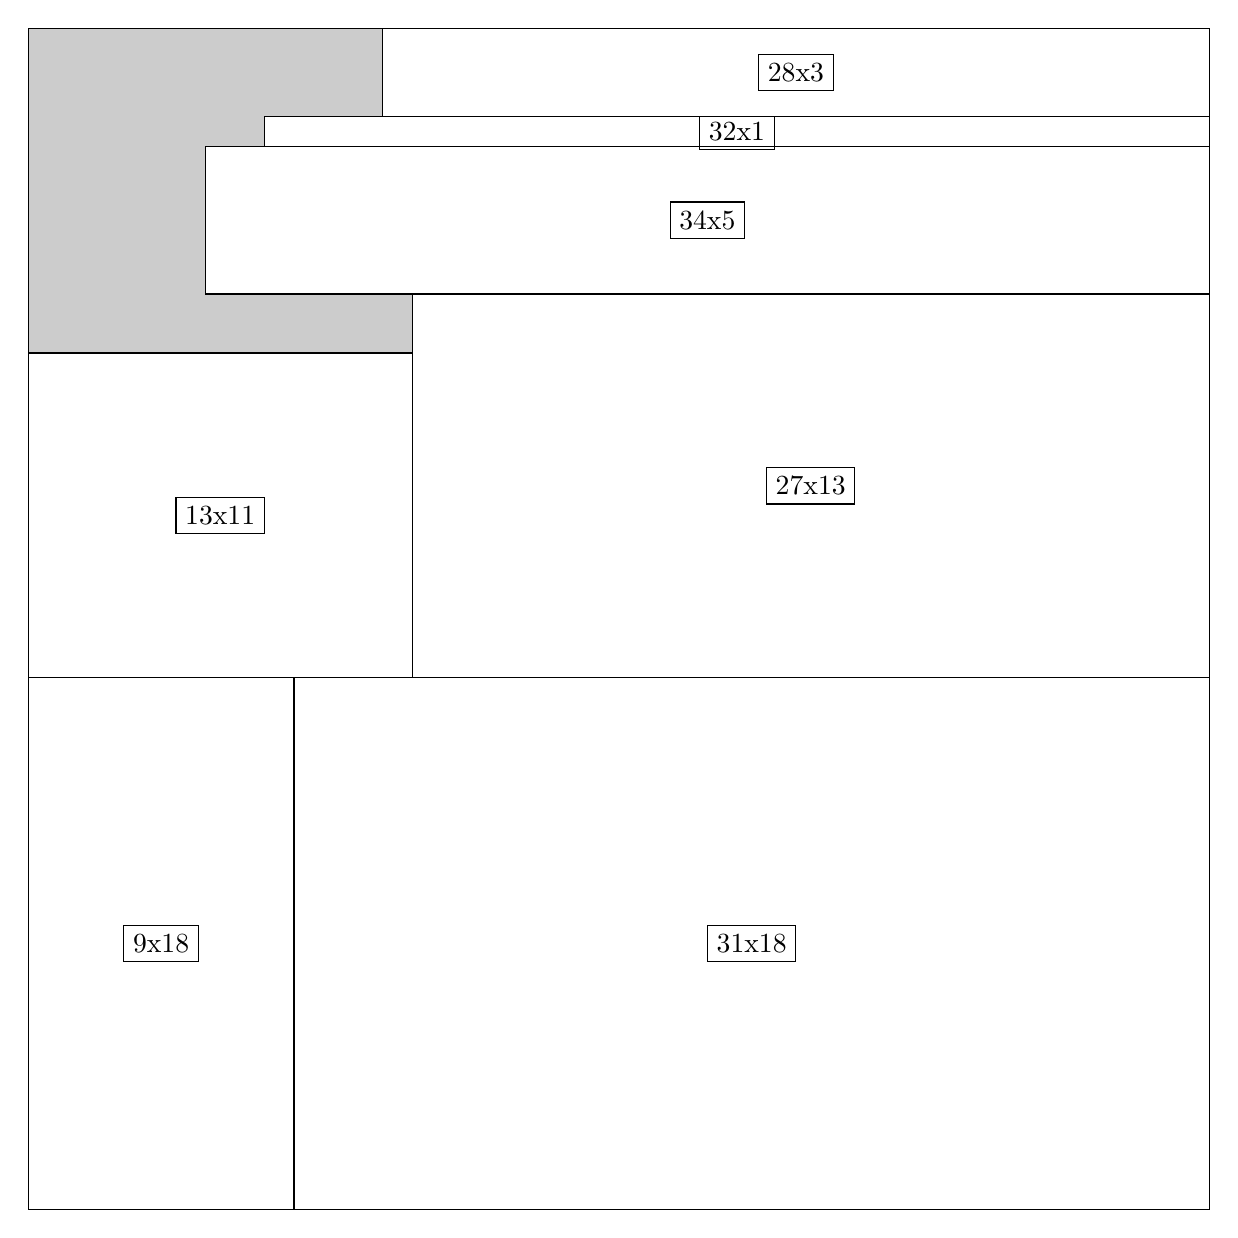
\begin{tikzpicture}[shorten >=1pt,scale=1.0,every node/.style={scale=1.0},->]
\tikzstyle{vertex}=[circle,fill=black!25,minimum size=14pt,inner sep=0pt]
\filldraw[fill=gray!40!white, draw=black] (0,0) rectangle (15.0,15.0);
\foreach \name/\x/\y/\w/\h in {31x18/3.375/0.0/11.625/6.75,9x18/0.0/0.0/3.375/6.75,27x13/4.875/6.75/10.125/4.875,13x11/0.0/6.75/4.875/4.125,34x5/2.25/11.625/12.75/1.875,32x1/3.0/13.5/12.0/0.375,28x3/4.5/13.875/10.5/1.125}
\filldraw[fill=white!40!white, draw=black] (\x,\y) rectangle node[draw] (\name) {\name} ++(\w,\h);
\end{tikzpicture}


w =31 , h =18 , x =9 , y =0 , v =558
\par
w =9 , h =18 , x =0 , y =0 , v =162
\par
w =27 , h =13 , x =13 , y =18 , v =351
\par
w =13 , h =11 , x =0 , y =18 , v =143
\par
w =34 , h =5 , x =6 , y =31 , v =170
\par
w =32 , h =1 , x =8 , y =36 , v =32
\par
w =28 , h =3 , x =12 , y =37 , v =84
\par
\newpage


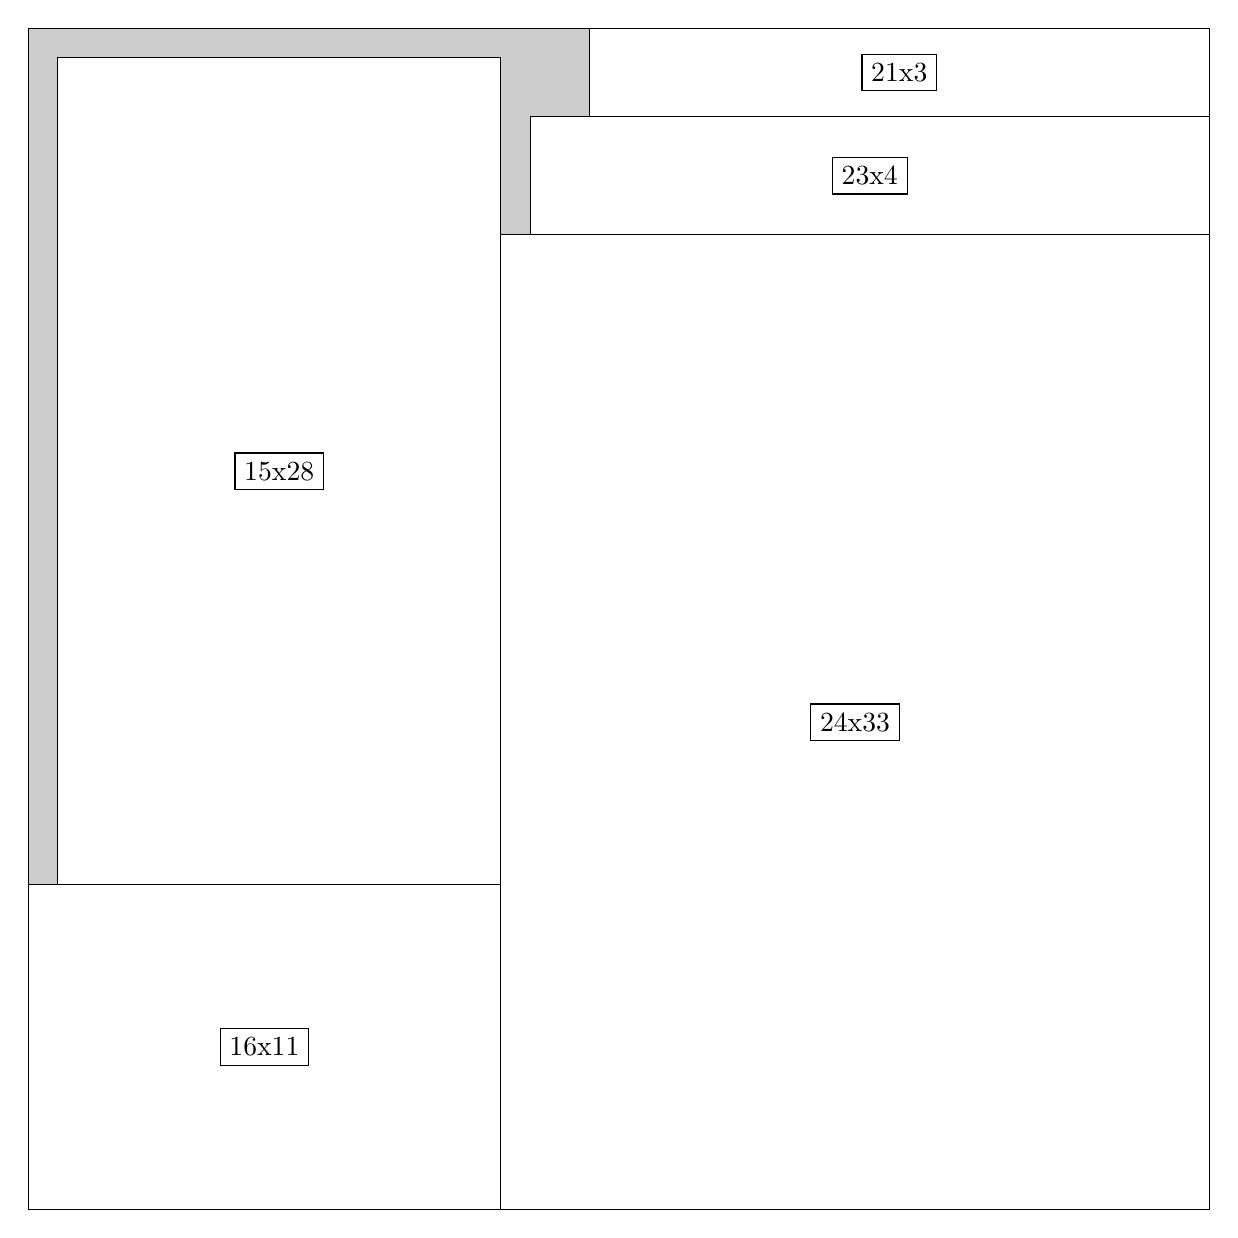
\begin{tikzpicture}[shorten >=1pt,scale=1.0,every node/.style={scale=1.0},->]
\tikzstyle{vertex}=[circle,fill=black!25,minimum size=14pt,inner sep=0pt]
\filldraw[fill=gray!40!white, draw=black] (0,0) rectangle (15.0,15.0);
\foreach \name/\x/\y/\w/\h in {24x33/6.0/0.0/9.0/12.375,23x4/6.375/12.375/8.625/1.5,21x3/7.125/13.875/7.875/1.125,16x11/0.0/0.0/6.0/4.125,15x28/0.375/4.125/5.625/10.5}
\filldraw[fill=white!40!white, draw=black] (\x,\y) rectangle node[draw] (\name) {\name} ++(\w,\h);
\end{tikzpicture}


w =24 , h =33 , x =16 , y =0 , v =792
\par
w =23 , h =4 , x =17 , y =33 , v =92
\par
w =21 , h =3 , x =19 , y =37 , v =63
\par
w =16 , h =11 , x =0 , y =0 , v =176
\par
w =15 , h =28 , x =1 , y =11 , v =420
\par
\newpage


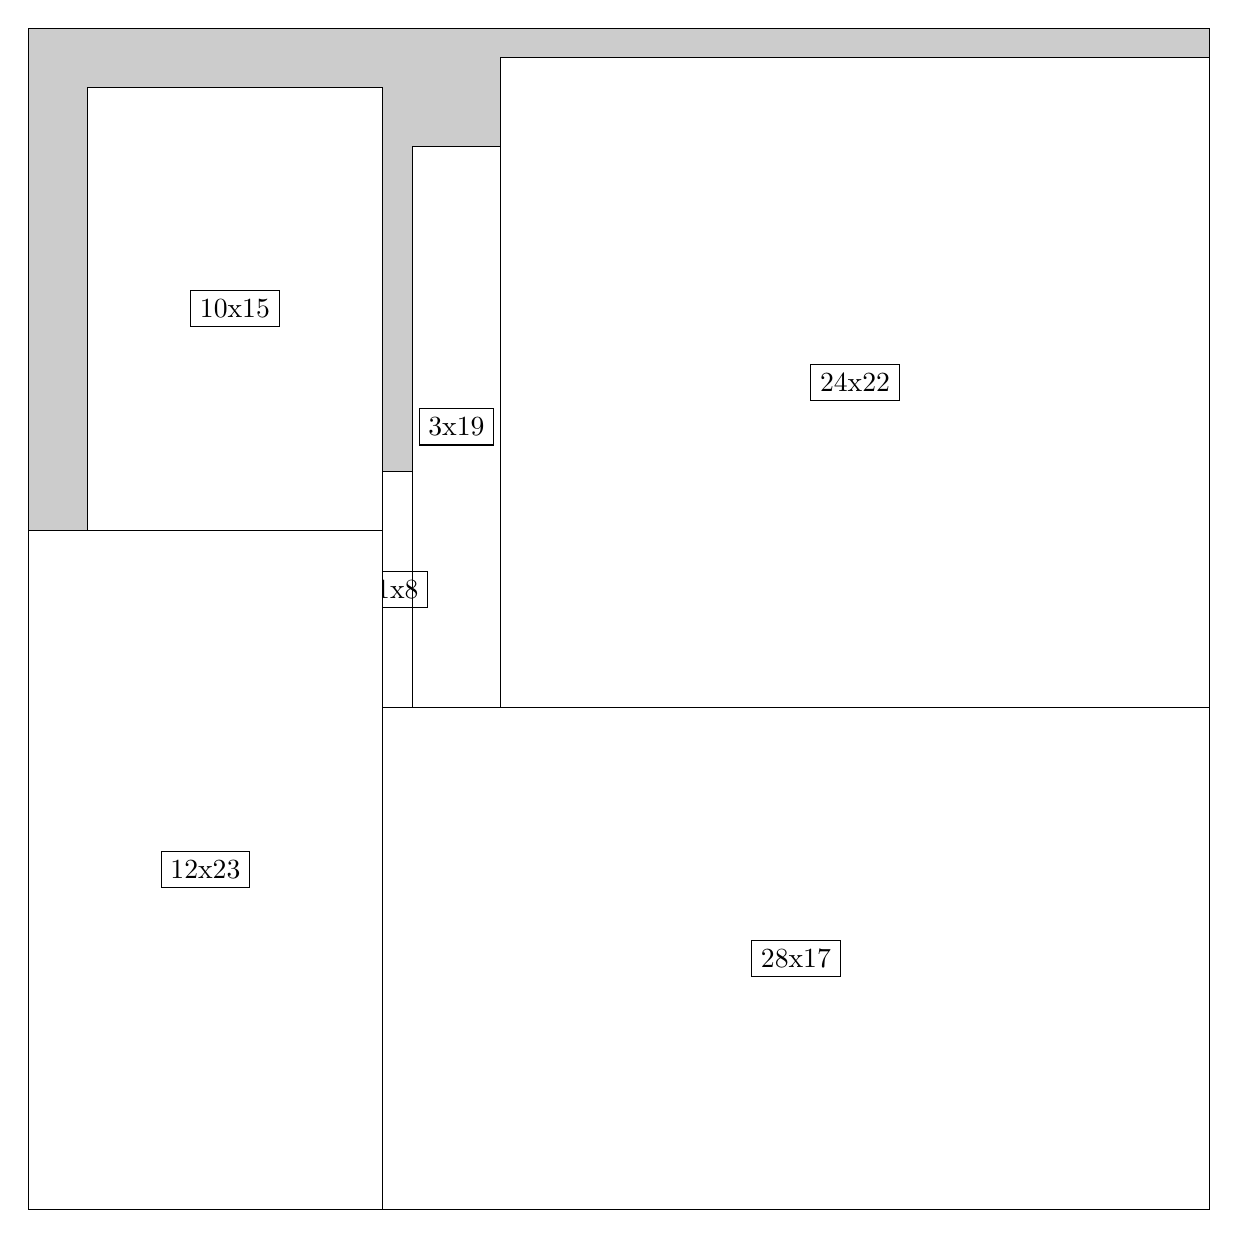
\begin{tikzpicture}[shorten >=1pt,scale=1.0,every node/.style={scale=1.0},->]
\tikzstyle{vertex}=[circle,fill=black!25,minimum size=14pt,inner sep=0pt]
\filldraw[fill=gray!40!white, draw=black] (0,0) rectangle (15.0,15.0);
\foreach \name/\x/\y/\w/\h in {28x17/4.5/0.0/10.5/6.375,24x22/6.0/6.375/9.0/8.25,3x19/4.875/6.375/1.125/7.125,1x8/4.5/6.375/0.375/3.0,12x23/0.0/0.0/4.5/8.625,10x15/0.75/8.625/3.75/5.625}
\filldraw[fill=white!40!white, draw=black] (\x,\y) rectangle node[draw] (\name) {\name} ++(\w,\h);
\end{tikzpicture}


w =28 , h =17 , x =12 , y =0 , v =476
\par
w =24 , h =22 , x =16 , y =17 , v =528
\par
w =3 , h =19 , x =13 , y =17 , v =57
\par
w =1 , h =8 , x =12 , y =17 , v =8
\par
w =12 , h =23 , x =0 , y =0 , v =276
\par
w =10 , h =15 , x =2 , y =23 , v =150
\par
\newpage


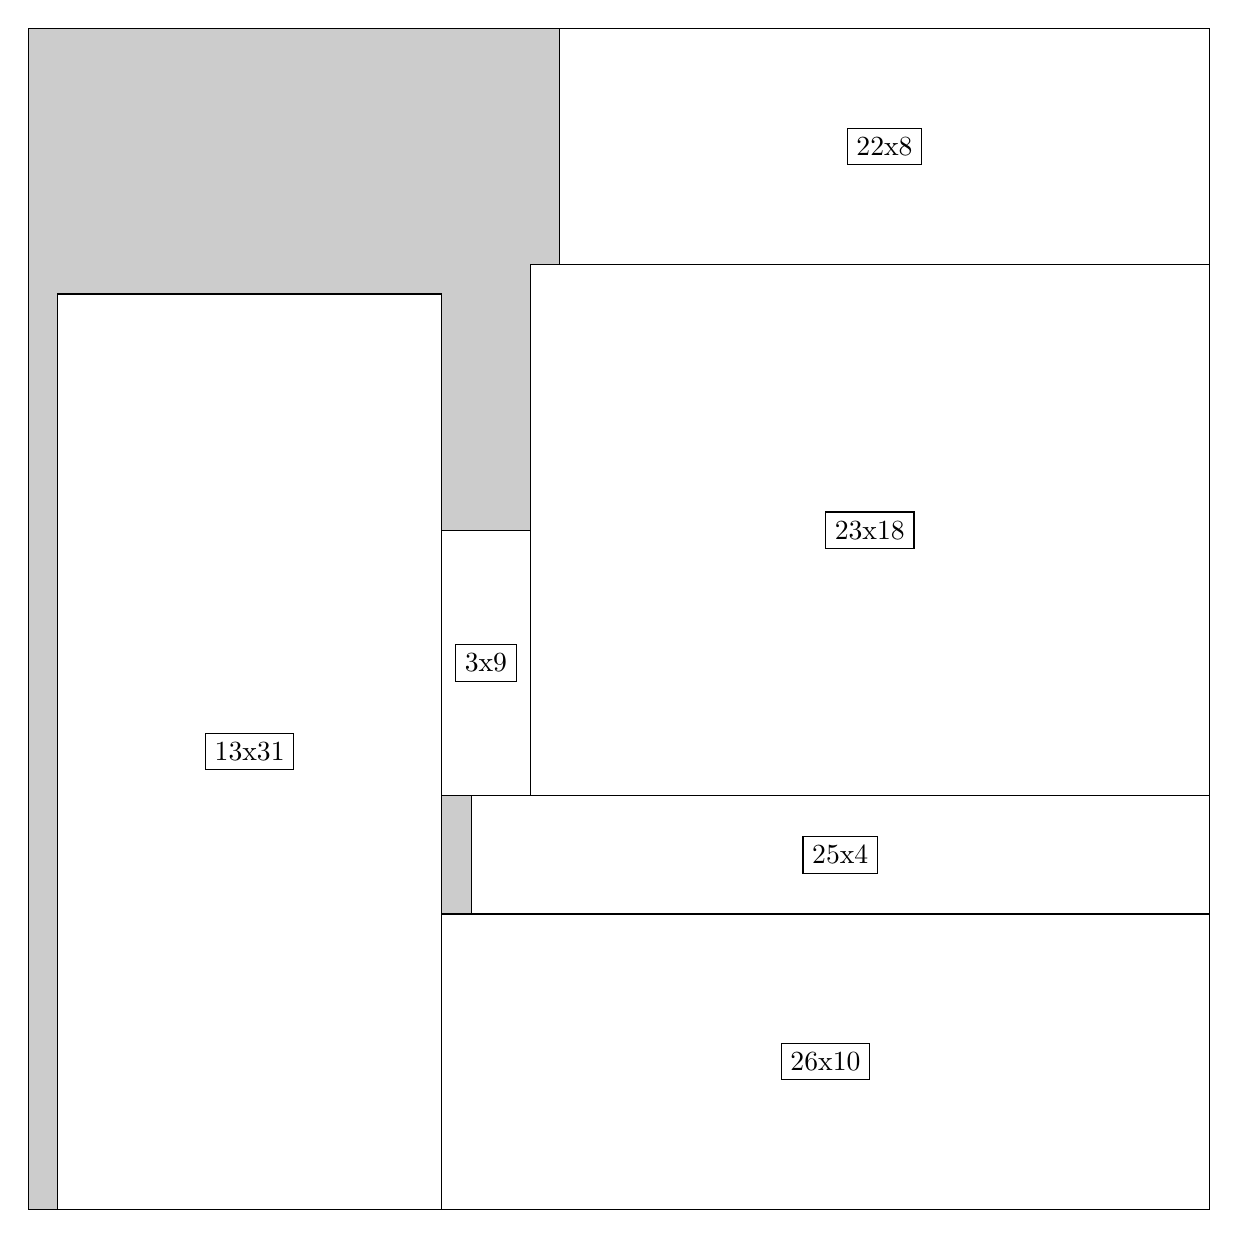
\begin{tikzpicture}[shorten >=1pt,scale=1.0,every node/.style={scale=1.0},->]
\tikzstyle{vertex}=[circle,fill=black!25,minimum size=14pt,inner sep=0pt]
\filldraw[fill=gray!40!white, draw=black] (0,0) rectangle (15.0,15.0);
\foreach \name/\x/\y/\w/\h in {26x10/5.25/0.0/9.75/3.75,25x4/5.625/3.75/9.375/1.5,23x18/6.375/5.25/8.625/6.75,3x9/5.25/5.25/1.125/3.375,22x8/6.75/12.0/8.25/3.0,13x31/0.375/0.0/4.875/11.625}
\filldraw[fill=white!40!white, draw=black] (\x,\y) rectangle node[draw] (\name) {\name} ++(\w,\h);
\end{tikzpicture}


w =26 , h =10 , x =14 , y =0 , v =260
\par
w =25 , h =4 , x =15 , y =10 , v =100
\par
w =23 , h =18 , x =17 , y =14 , v =414
\par
w =3 , h =9 , x =14 , y =14 , v =27
\par
w =22 , h =8 , x =18 , y =32 , v =176
\par
w =13 , h =31 , x =1 , y =0 , v =403
\par
\newpage


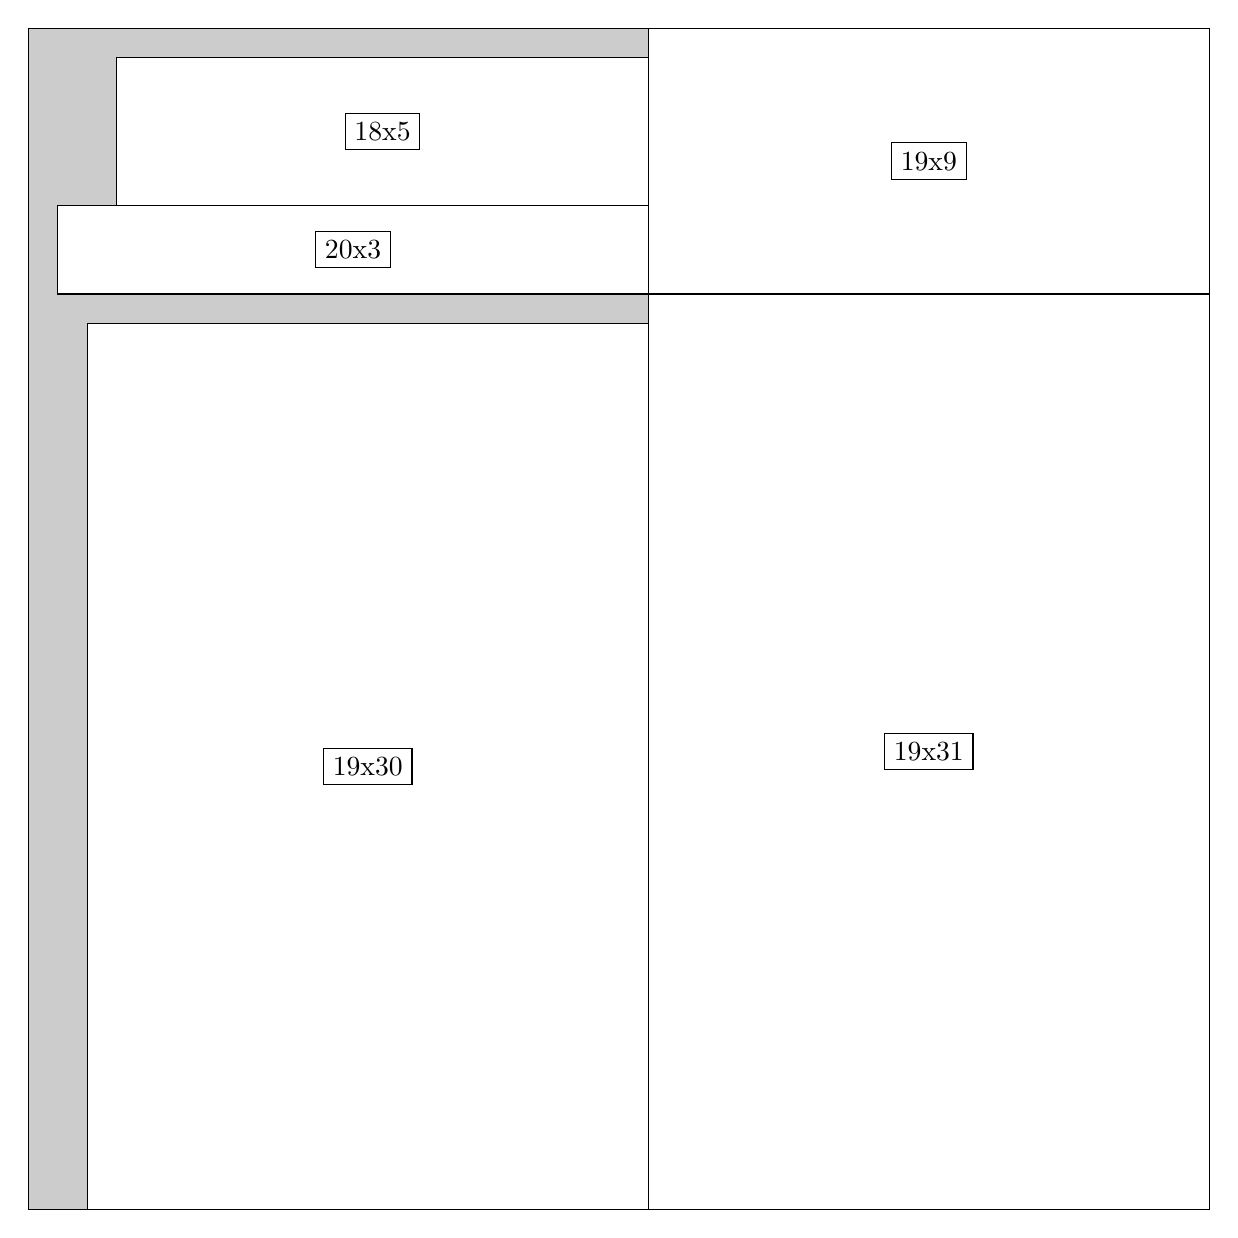
\begin{tikzpicture}[shorten >=1pt,scale=1.0,every node/.style={scale=1.0},->]
\tikzstyle{vertex}=[circle,fill=black!25,minimum size=14pt,inner sep=0pt]
\filldraw[fill=gray!40!white, draw=black] (0,0) rectangle (15.0,15.0);
\foreach \name/\x/\y/\w/\h in {19x31/7.875/0.0/7.125/11.625,19x30/0.75/0.0/7.125/11.25,19x9/7.875/11.625/7.125/3.375,20x3/0.375/11.625/7.5/1.125,18x5/1.125/12.75/6.75/1.875}
\filldraw[fill=white!40!white, draw=black] (\x,\y) rectangle node[draw] (\name) {\name} ++(\w,\h);
\end{tikzpicture}


w =19 , h =31 , x =21 , y =0 , v =589
\par
w =19 , h =30 , x =2 , y =0 , v =570
\par
w =19 , h =9 , x =21 , y =31 , v =171
\par
w =20 , h =3 , x =1 , y =31 , v =60
\par
w =18 , h =5 , x =3 , y =34 , v =90
\par
\newpage


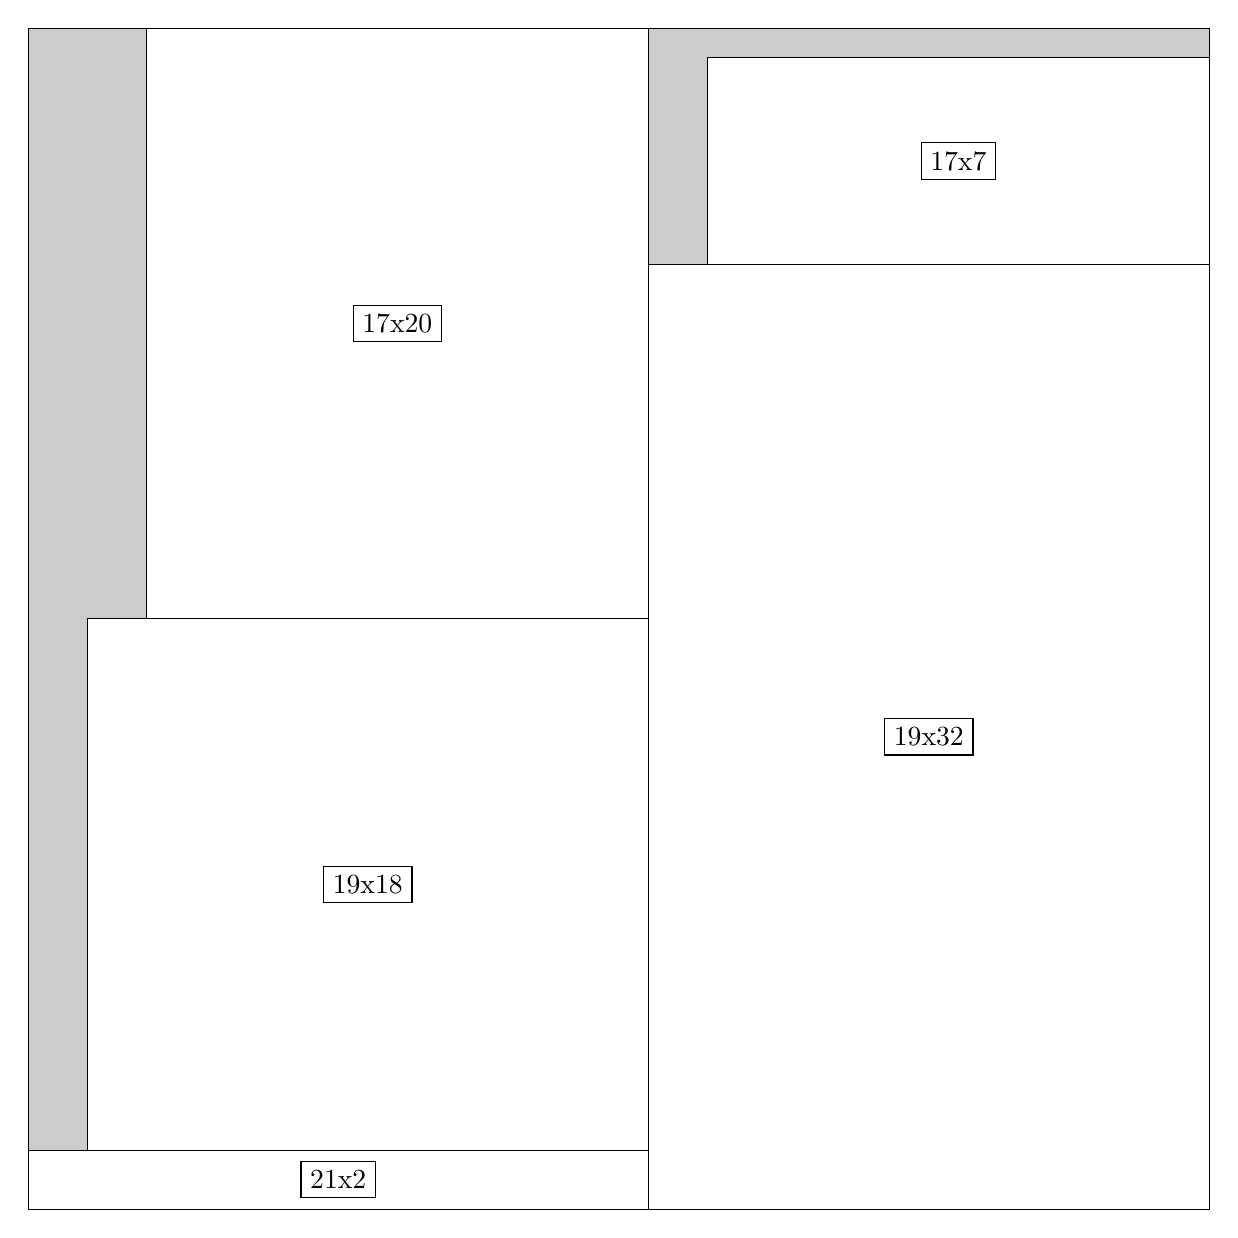
\begin{tikzpicture}[shorten >=1pt,scale=1.0,every node/.style={scale=1.0},->]
\tikzstyle{vertex}=[circle,fill=black!25,minimum size=14pt,inner sep=0pt]
\filldraw[fill=gray!40!white, draw=black] (0,0) rectangle (15.0,15.0);
\foreach \name/\x/\y/\w/\h in {19x32/7.875/0.0/7.125/12.0,17x7/8.625/12.0/6.375/2.625,21x2/0.0/0.0/7.875/0.75,19x18/0.75/0.75/7.125/6.75,17x20/1.5/7.5/6.375/7.5}
\filldraw[fill=white!40!white, draw=black] (\x,\y) rectangle node[draw] (\name) {\name} ++(\w,\h);
\end{tikzpicture}


w =19 , h =32 , x =21 , y =0 , v =608
\par
w =17 , h =7 , x =23 , y =32 , v =119
\par
w =21 , h =2 , x =0 , y =0 , v =42
\par
w =19 , h =18 , x =2 , y =2 , v =342
\par
w =17 , h =20 , x =4 , y =20 , v =340
\par
\newpage


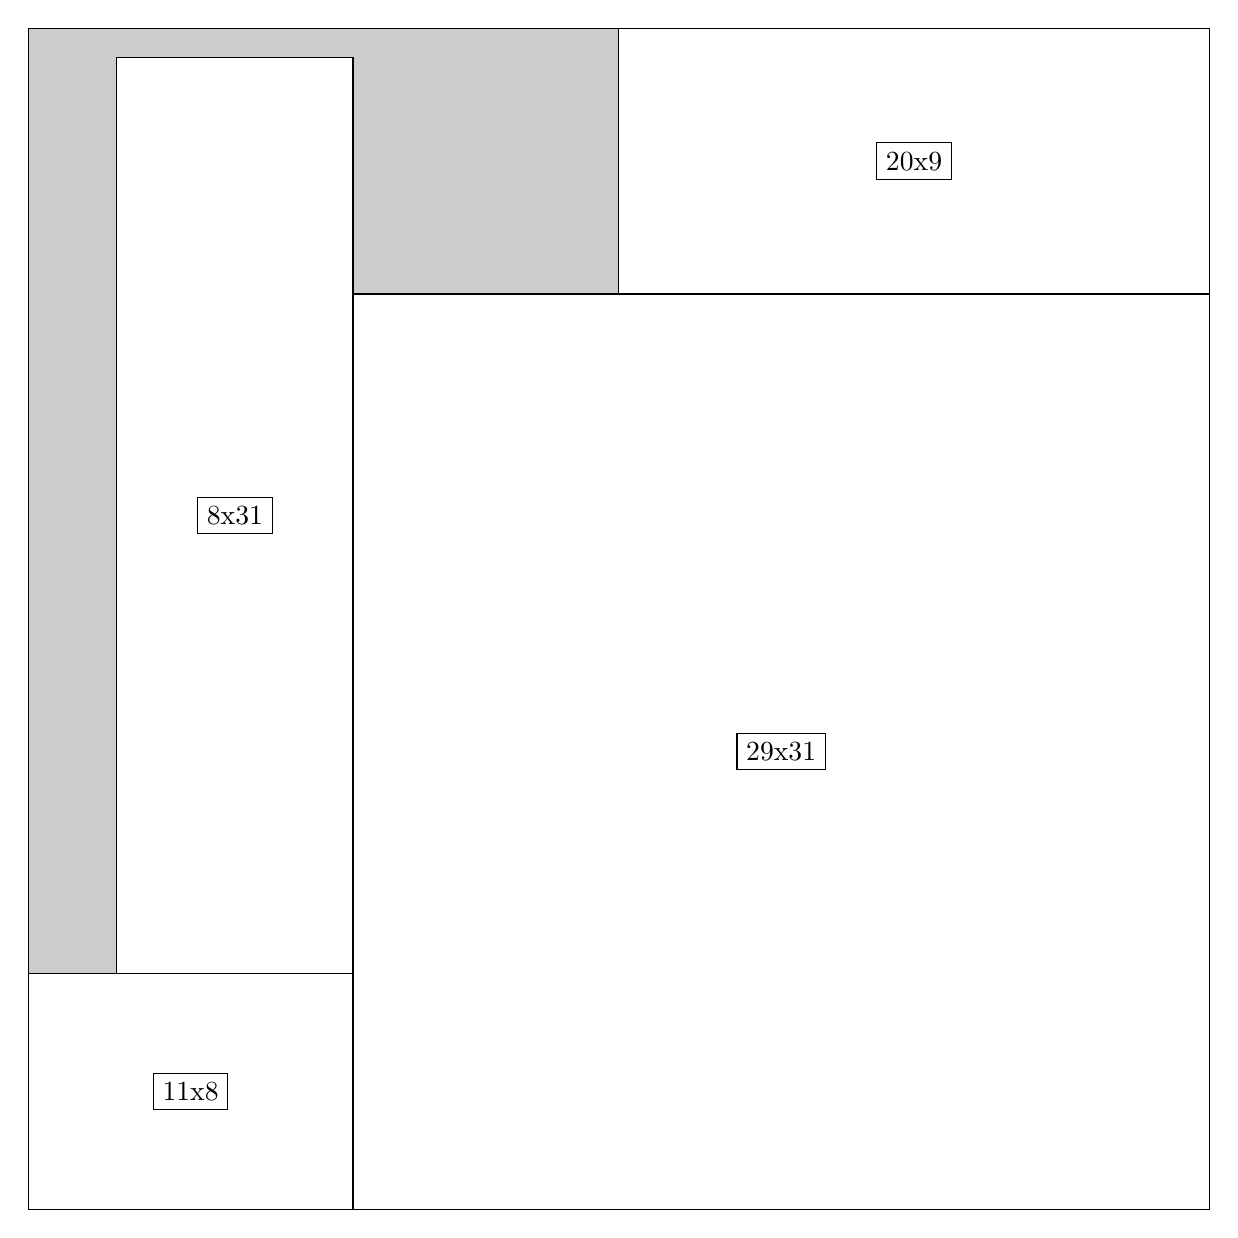
\begin{tikzpicture}[shorten >=1pt,scale=1.0,every node/.style={scale=1.0},->]
\tikzstyle{vertex}=[circle,fill=black!25,minimum size=14pt,inner sep=0pt]
\filldraw[fill=gray!40!white, draw=black] (0,0) rectangle (15.0,15.0);
\foreach \name/\x/\y/\w/\h in {29x31/4.125/0.0/10.875/11.625,20x9/7.5/11.625/7.5/3.375,11x8/0.0/0.0/4.125/3.0,8x31/1.125/3.0/3.0/11.625}
\filldraw[fill=white!40!white, draw=black] (\x,\y) rectangle node[draw] (\name) {\name} ++(\w,\h);
\end{tikzpicture}


w =29 , h =31 , x =11 , y =0 , v =899
\par
w =20 , h =9 , x =20 , y =31 , v =180
\par
w =11 , h =8 , x =0 , y =0 , v =88
\par
w =8 , h =31 , x =3 , y =8 , v =248
\par
\newpage


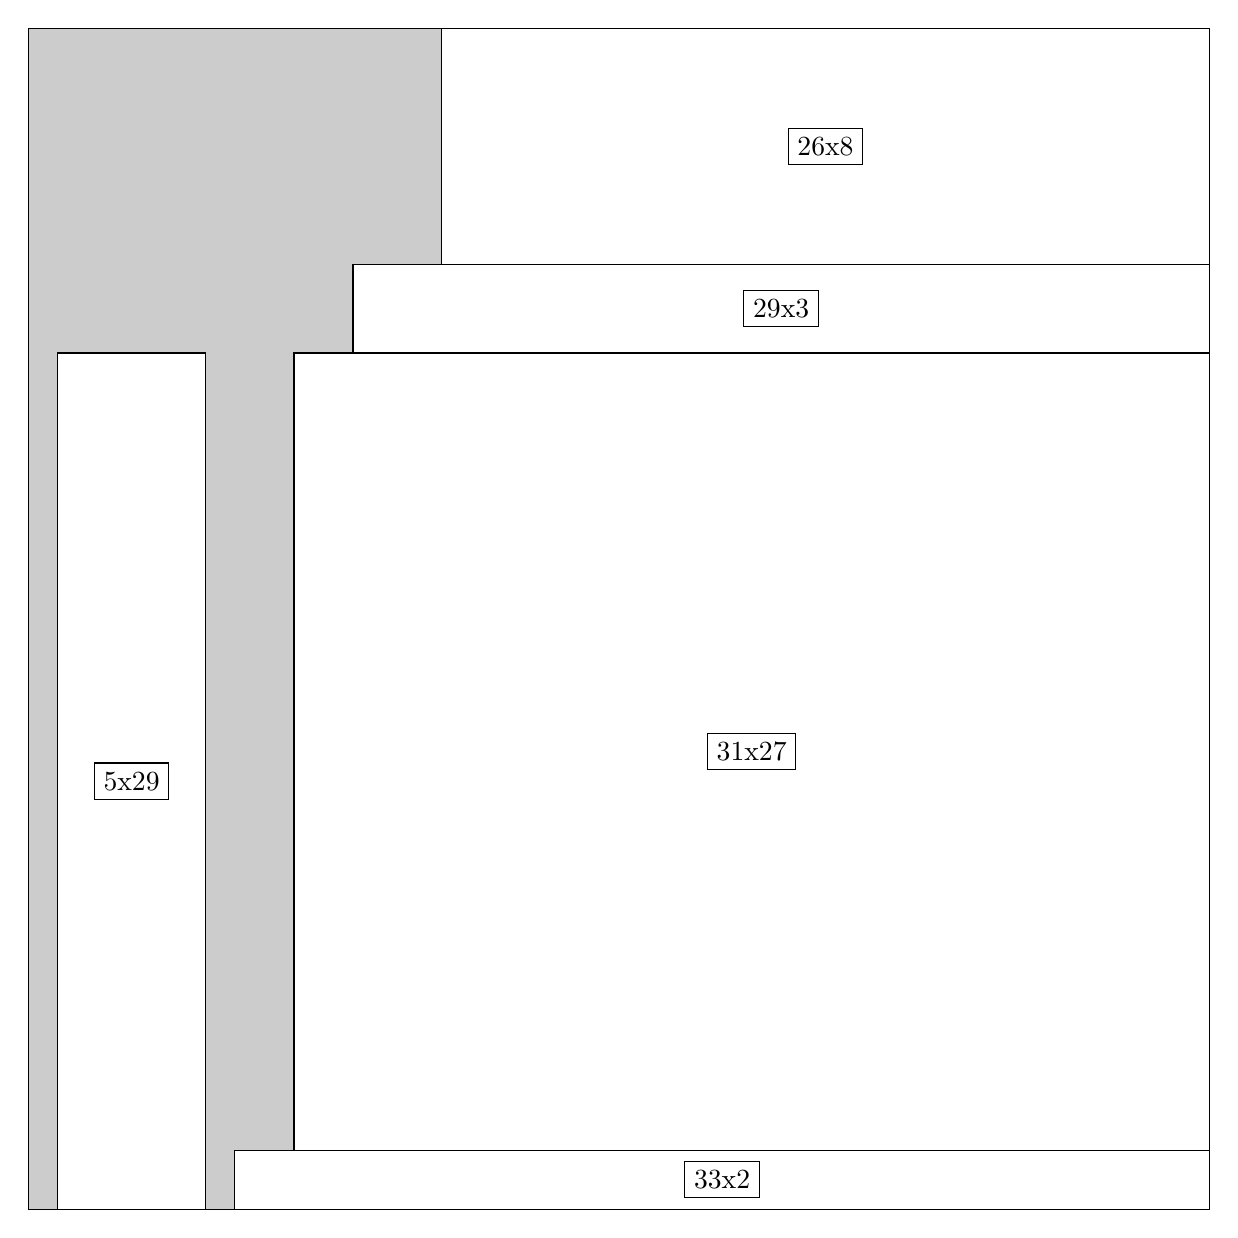
\begin{tikzpicture}[shorten >=1pt,scale=1.0,every node/.style={scale=1.0},->]
\tikzstyle{vertex}=[circle,fill=black!25,minimum size=14pt,inner sep=0pt]
\filldraw[fill=gray!40!white, draw=black] (0,0) rectangle (15.0,15.0);
\foreach \name/\x/\y/\w/\h in {33x2/2.625/0.0/12.375/0.75,31x27/3.375/0.75/11.625/10.125,29x3/4.125/10.875/10.875/1.125,26x8/5.25/12.0/9.75/3.0,5x29/0.375/0.0/1.875/10.875}
\filldraw[fill=white!40!white, draw=black] (\x,\y) rectangle node[draw] (\name) {\name} ++(\w,\h);
\end{tikzpicture}


w =33 , h =2 , x =7 , y =0 , v =66
\par
w =31 , h =27 , x =9 , y =2 , v =837
\par
w =29 , h =3 , x =11 , y =29 , v =87
\par
w =26 , h =8 , x =14 , y =32 , v =208
\par
w =5 , h =29 , x =1 , y =0 , v =145
\par
\newpage


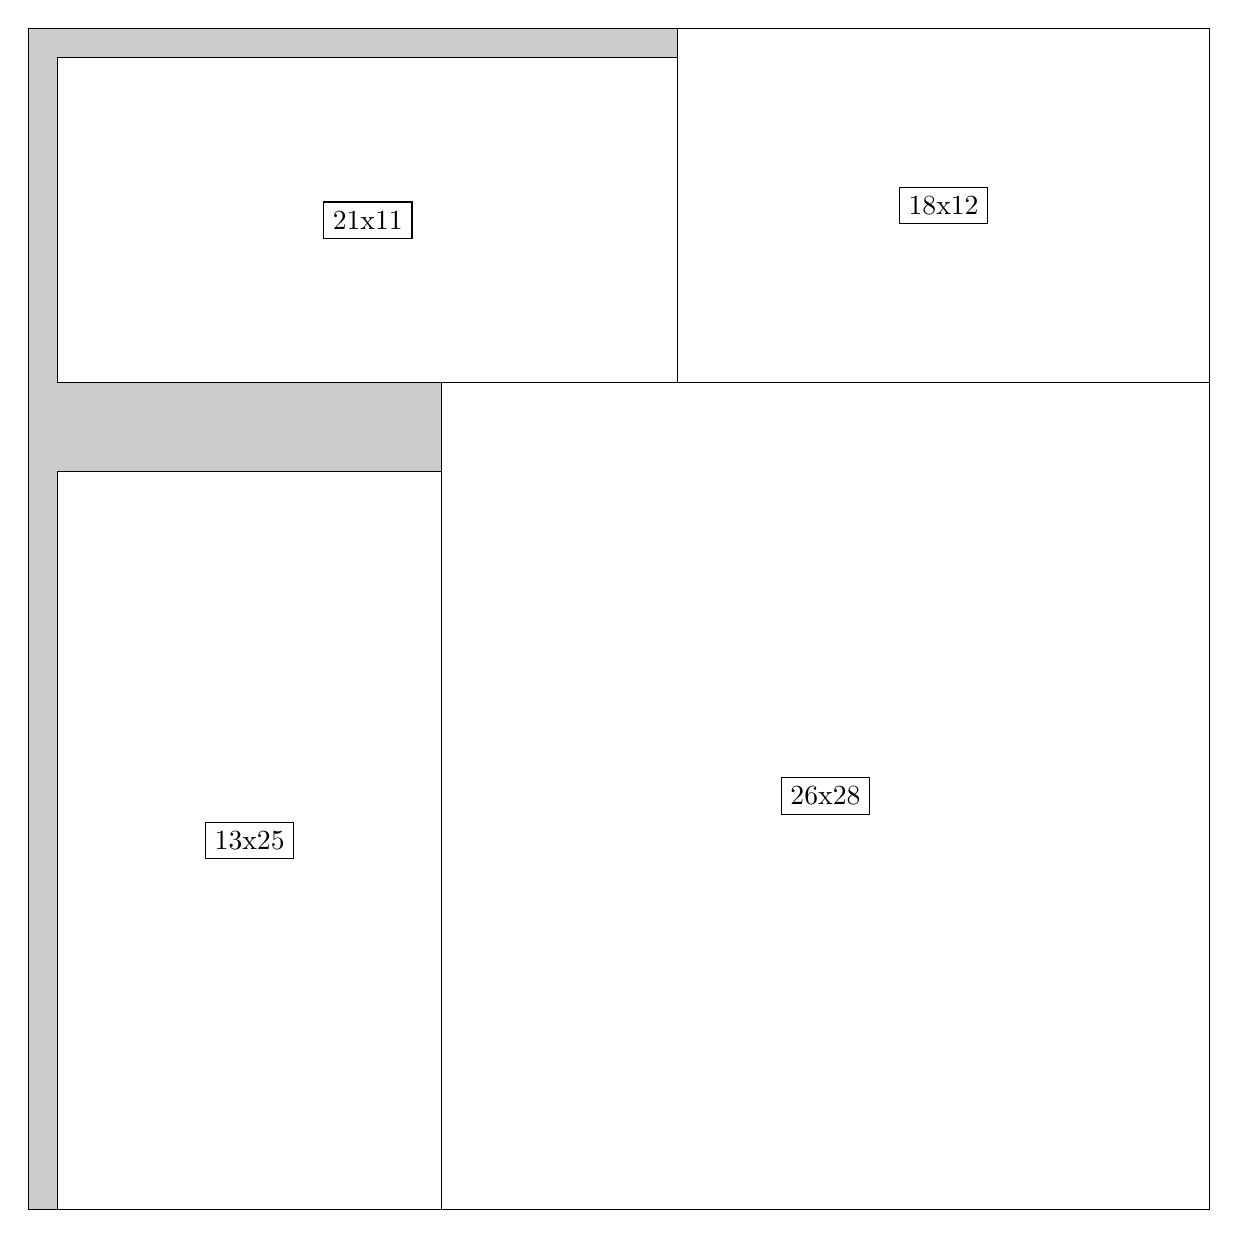
\begin{tikzpicture}[shorten >=1pt,scale=1.0,every node/.style={scale=1.0},->]
\tikzstyle{vertex}=[circle,fill=black!25,minimum size=14pt,inner sep=0pt]
\filldraw[fill=gray!40!white, draw=black] (0,0) rectangle (15.0,15.0);
\foreach \name/\x/\y/\w/\h in {26x28/5.25/0.0/9.75/10.5,13x25/0.375/0.0/4.875/9.375,18x12/8.25/10.5/6.75/4.5,21x11/0.375/10.5/7.875/4.125}
\filldraw[fill=white!40!white, draw=black] (\x,\y) rectangle node[draw] (\name) {\name} ++(\w,\h);
\end{tikzpicture}


w =26 , h =28 , x =14 , y =0 , v =728
\par
w =13 , h =25 , x =1 , y =0 , v =325
\par
w =18 , h =12 , x =22 , y =28 , v =216
\par
w =21 , h =11 , x =1 , y =28 , v =231
\par
\newpage


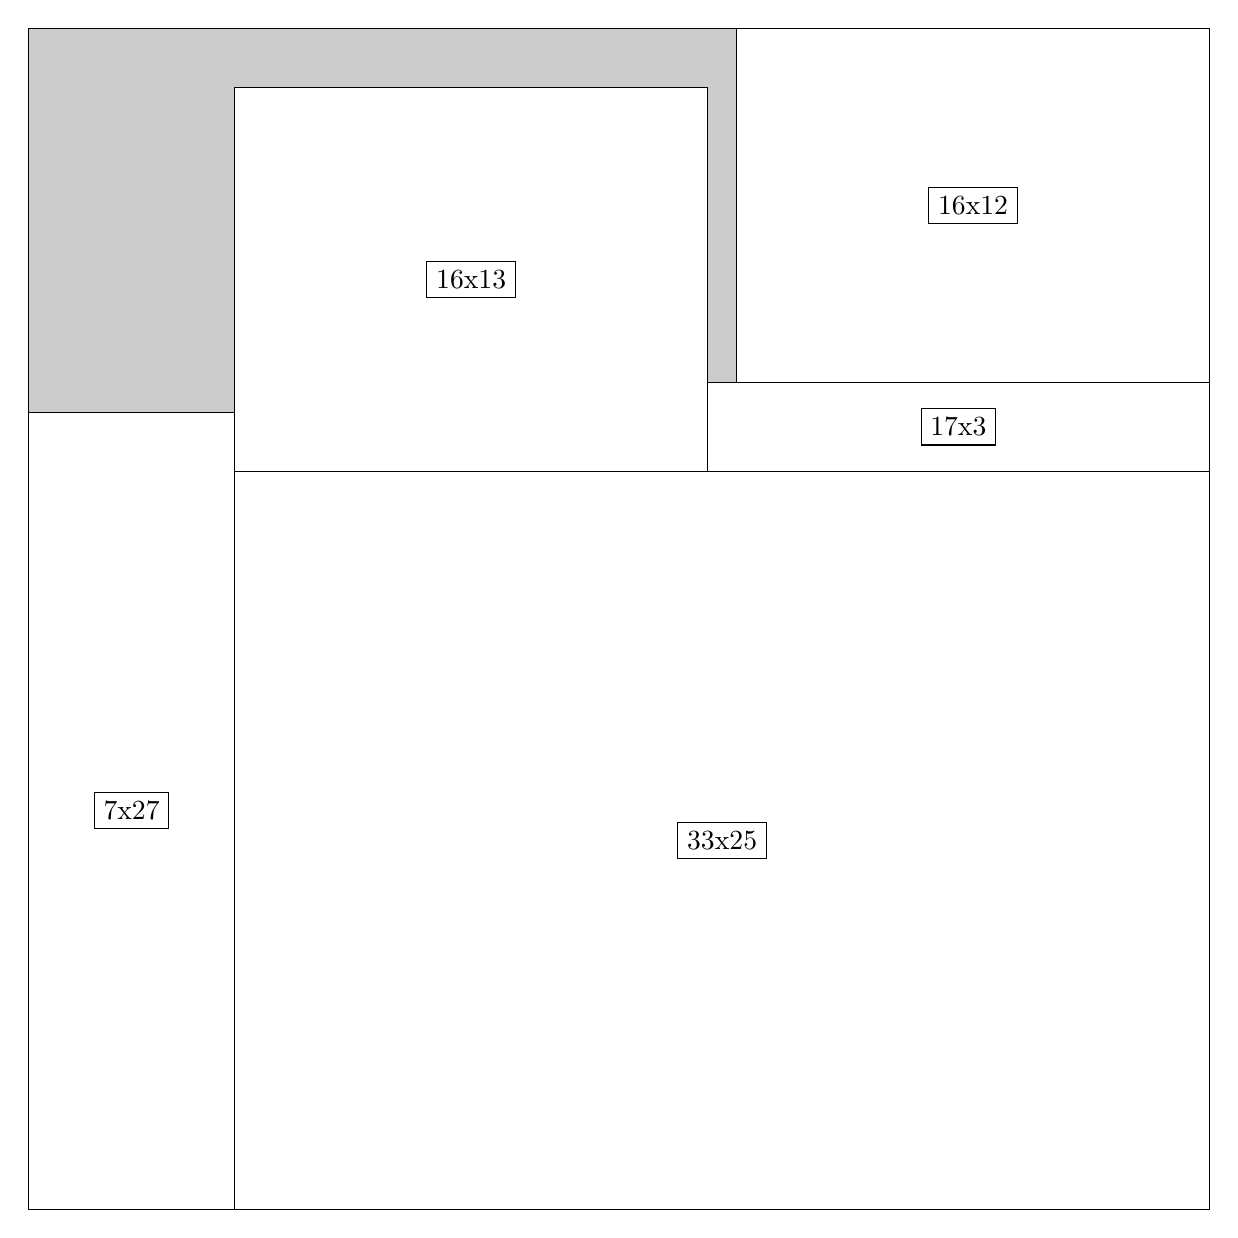
\begin{tikzpicture}[shorten >=1pt,scale=1.0,every node/.style={scale=1.0},->]
\tikzstyle{vertex}=[circle,fill=black!25,minimum size=14pt,inner sep=0pt]
\filldraw[fill=gray!40!white, draw=black] (0,0) rectangle (15.0,15.0);
\foreach \name/\x/\y/\w/\h in {33x25/2.625/0.0/12.375/9.375,17x3/8.625/9.375/6.375/1.125,16x12/9.0/10.5/6.0/4.5,16x13/2.625/9.375/6.0/4.875,7x27/0.0/0.0/2.625/10.125}
\filldraw[fill=white!40!white, draw=black] (\x,\y) rectangle node[draw] (\name) {\name} ++(\w,\h);
\end{tikzpicture}


w =33 , h =25 , x =7 , y =0 , v =825
\par
w =17 , h =3 , x =23 , y =25 , v =51
\par
w =16 , h =12 , x =24 , y =28 , v =192
\par
w =16 , h =13 , x =7 , y =25 , v =208
\par
w =7 , h =27 , x =0 , y =0 , v =189
\par
\newpage


\begin{tikzpicture}[shorten >=1pt,scale=1.0,every node/.style={scale=1.0},->]
\tikzstyle{vertex}=[circle,fill=black!25,minimum size=14pt,inner sep=0pt]
\filldraw[fill=gray!40!white, draw=black] (0,0) rectangle (15.0,15.0);
\foreach \name/\x/\y/\w/\h in {19x33/7.875/0.0/7.125/12.375,17x33/1.5/0.0/6.375/12.375,4x32/0.0/0.0/1.5/12.0,33x7/2.625/12.375/12.375/2.625,2x7/1.875/12.375/0.75/2.625,4x6/0.375/12.375/1.5/2.25}
\filldraw[fill=white!40!white, draw=black] (\x,\y) rectangle node[draw] (\name) {\name} ++(\w,\h);
\end{tikzpicture}


w =19 , h =33 , x =21 , y =0 , v =627
\par
w =17 , h =33 , x =4 , y =0 , v =561
\par
w =4 , h =32 , x =0 , y =0 , v =128
\par
w =33 , h =7 , x =7 , y =33 , v =231
\par
w =2 , h =7 , x =5 , y =33 , v =14
\par
w =4 , h =6 , x =1 , y =33 , v =24
\par
\newpage


\end{document}